\section{Artificial Neural Networks}

With the explosion of the amount of collected data and the rapid development of computer hardware in the twenty-first century, deep learning techniques have been used extensively for solving different classes of problems.
Deep learning techniques are revolutionary in that they can automatically capture the relationship between the inputs and the outputs, allowing machines to perform complex tasks without having humans explicitly told them what to do.
These capabilities are empowered by the underlying \gls{ANN} architecture, allowing computing systems to mimic the functionality of biological neural networks, which comprise animal brains.
An \gls{ANN} simulates biological neural networks by having the ability to learn from experiences and examples.
This process works by using a set of inputs with known outputs.
The \gls{ANN} is then used to guess the outputs from the inputs.
The differences between the guess output values and the known output values indicate what changes need to be made to the \gls{ANN}.
These updates to the \gls{ANN} are done multiple times until the guess error is minimized or some criteria are met.
This process is now called \textit{supervised learning}.

\begin{figure}[h]
    \centering
    \begin{neuralnetwork}
        \newcommand{\nodex}[2]{$x_#2$}
        \newcommand{\nodefx}[2]{$f(x)$}
        \newcommand{\nodey}[2]{$y_#2$}

        \newcommand{\nodewfirstlayer}[1]{\ifnum0=#1 {} \else $w_#1$ \fi}
        \newcommand{\nodew}[4]{\ifnum0=#1 \nodewfirstlayer{#2} \else {} \fi}
        \setdefaultlinklabel{\nodew}

        \inputlayer[count=3, bias=true, text=\nodex]
        \outputlayer[count=1, bias=false, text=\nodefx]
        \linklayers
        \outputlayer[count=1, bias=false, text=\nodey]
        \linklayers
    \end{neuralnetwork}
    \caption{Graph representation of a perceptron described in \autoref{eq:perceptron}. $x_0$ is the bias $b$, and $x_{1-3}$ are the input signals.}
    \label{fig:perceptron}
\end{figure}

The idea for a computational model based on the brain was first proposed by \citeauthor{mcculloch1943logical} \cite{mcculloch1943logical} in \citeyear{mcculloch1943logical}.
They observed that nervous activity, neural events, and their relations could be demonstrated using propositional logic.
Later on, researchers had been building upon that idea to find more methods for artificially representing the brain.
In \citeyear{rosenblattPerceptronProbabilisticModel1958}, \citeauthor{rosenblattPerceptronProbabilisticModel1958} \cite{rosenblattPerceptronProbabilisticModel1958} introduced the concept of perceptrons which is considered the first \gls{ANN}.
Mathematically, a perceptron is expressed as
\begin{equation}
    f(x) = \begin{cases}
        1 & \textrm{if}\ w \cdot x + b > 0 \\
        0 & \textrm{otherwise}
    \end{cases}
    \label{eq:perceptron}
\end{equation}
where $w$ and $x$ are vectors of real value, $w \cdot x = \sum_{i=1}^m{w_i x_i}$ is the dot product between the two vectors, and $b$ is the bias for shifting the decision boundary.
The perceptron is illustrated in \autoref{fig:perceptron}.
This initial version of \gls{ANN} only works with classification problems in which the classes are linearly separable.

Nowadays, neural networks are highly complex because of the considerably higher computing power and the developments of special-purpose hardware, such as the \gls{GPU}.
Multiple different architectures of neural networks exist, a non-exhaustive list includes: \glspl{CNN} are typically used for processing images or other two-dimensional data \cite{lecunBackpropagationAppliedHandwritten1989}; \glspl{LSTM} solve the vanishing gradient problem and have the ability to handle data with a mix of low and high frequencies \cite{hochreiterLongShortTermMemory1997}; \glspl{GAN} are designed to have competing \glspl{ANN} on tasks such as playing a game \cite{silverMasteringChessShogi2017}.

\begin{figure}[h]
    \centering
    \begin{neuralnetwork}
        \newcommand{\nodex}[2]{$x_#2$}
        \newcommand{\nodey}[2]{$y_#2$}

        \inputlayer[count=3, bias=false, title={Input\\layer}, text=\nodex]
        \hiddenlayer[count=4, bias=false, title={Hidden\\layer}]
        \linklayers[title=$W_1$]
        \hiddenlayer[count=4, bias=false, title={Hidden\\layer}]
        \linklayers[title=$W_2$]
        \outputlayer[count=2, bias=false, title={Output\\layer}, text=\nodey]
        \linklayers[title=$W_3$]
    \end{neuralnetwork}
    \caption{Graph representation of a multi-layer perceptron with four layers}
    \label{fig:multi-layer-perceptron}
\end{figure}

\gls{MLP} is a network that composes multiple nodes, called artificial neurons.
These nodes in the network form a directed weighted graph, where each node can take input signals from nodes in the previous layer, performs some calculation and sends the results to nodes in the subsequent layer.
In this configuration, an \gls{MLP} can be thought of as multiple perceptrons that are organized into layers.
The first layer in the network is called the input layer, and the last layer is called the output layer; any layers in-between are called hidden layers.
Commonly, the term \gls{MLP} is used to describe an \gls{ANN} where each node in a layer connects to all of the nodes in the subsequent layer, and nodes can only connect from one layer to the immediately subsequent layer.
Other terms for this are fully connected \gls{ANN} or densely connected \gls{ANN}.
Additionally, an \gls{MLP} is a type of feed-forward \gls{ANN}, i.e., signals in this network are passed from one layer to another in one direction only.
The counterpart of this is the feedback \gls{ANN}.
In a feedback \gls{ANN}, signals can flow in any direction, as can be seen in \gls{RNN}.
Mathematically, each node in an \gls{MLP} computes the following values
\begin{align*}
    a_i^k &= b_i^k + \sum_{j=1}^{r_{k-1}} w_{ij}^k z_j^{k-1} \\
    z_i^k &= \phi (a_i^k),
\end{align*}
where $\phi$ is a nonlinear function that gets applied to the output $a_i^k$ of layer $k$, $w_{ij}^k$ is the weight that maps the node $j$ in layer $k - 1$ to node $i$ in layer $k$, $b_i$ is the bias term for node $i$ in layer $k$, $z_i^k$ is the product sum plus bias for node $i$ in layer $k$, $a_i^k$ is the activated output of node $i$ in layer $k$, and $r_k$ is the number of nodes in layer $k$.
This computation is similar to perceptron, excepting the function $\phi$, called the \textit{activation function}.
Let $n$ be the depth of a network, i.e., the number of layers having adjustable weights, and $X$ be the vectors of input signals.
Let $W_i$, $b_i$, and $\phi_i$ be the vector of weights, vector of bias terms, and the activation function for each layer, where $i \in [1, n]$.
An \gls{MLP} is expressing the following function
\begin{equation*}
    g(X) = \phi_n(W_n \phi_{n - 1}(\cdots (W_2 \phi_1(W_1 X + b_1) + b_2) + \cdots) + b_n).
\end{equation*}

\subsection{Training Artificial Neural Networks}
\label{sec:training-artificial-neural-networks}

\begin{algorithm}
    \caption{Batch gradient descent for training \gls{ANN}. The learning rate $\eta$ influences how much the weights and bias terms are updated in each iteration.}
    \label{alg:ann-training}
    \begin{algorithmic}
        \State $\mathcal{D} \gets \{(x_t, y_t)\ |\ t \in [1, n]\}$
        \Comment{Get training data with $n$ samples}
        \State $\eta \gets \text{learning rate}$
        \Comment{Choose a learning rate}
        \State $W \gets \text{random values}$
        \Comment{Randomly initailize the weights}
        \State $b \gets \text{random values}$
        \Comment{Randomly initailize the bias terms}
        \While{criteria are not met}
            \State $\Delta W \gets 0$
            \Comment{Set the accumulated gradients w.r.t to each weight to zero}
            \State $\Delta b \gets 0$
            \Comment{Set the accumulated gradients w.r.t to each bias terms to zero}
            \ForAll{$(x, y) \in \mathcal{D}$}
            \Comment{Go through all training data}
                \State $\hat{y} \gets \mathcal{NN}_{W, b}(x)$
                \Comment{Compute the neural network output}
                \State $E \gets \mathcal{L}(\hat{y}, y)$
                \Comment{Compute the loss value}
                \State $\Delta W \gets \Delta W + \eta \frac{\partial E}{\partial W}$
                \Comment{Accumulate the loss gradients w.r.t to each weight}
                \State $\Delta b \gets \Delta b + \eta \frac{\partial E}{\partial b}$
                \Comment{Accumulate the loss gradients w.r.t to each bias term}
            \EndFor
            \State $W \gets W - \Delta W$
            \Comment{Update all the weights with the accumulated gradients}
            \State $b \gets b - \Delta b$
            \Comment{Update all the bias terms with the accumulated gradients}
        \EndWhile
    \end{algorithmic}
\end{algorithm}


\glspl{MLP} and other \glspl{ANN} can be used for various tasks because they are universal approximators \cite{cybenkotApproximationSuperpositionsSigmoidal, hornikApproximationCapabilitiesMultilayer1991, hornikMultilayerFeedforwardNetworks1989}.
That means a sufficiently large \gls{ANN} with an arbitrary number of nodes can reasonably approximate any function $f: \mathbb{R}^M \mapsto \mathbb{R}^N$, given that appropriate weights can be found.
However, the exact method for finding suitable weights is not defined.
Commonly, the fitting weights are learned by \glspl{ANN} through the back-propagation algorithm \cite{rumelhartLearningRepresentationsBackpropagating1986} and the gradient descent optimization technique \cite{ruderOverviewGradientDescent2017}.
A simple training procedure for most \glspl{ANN} is given in \autoref{alg:ann-training}.
Back-propagation is the algorithm for finding the gradients of a loss function with respect to the network's weights.
A loss function measures how large the error is between the \gls{ANN}'s guess and the true value.
One choice is the \gls{MSE} $\mathcal{L} = \frac{1}{N} \sum_{i=1}^N (\hat{y} - y)^2$
The algorithm calculates the gradients starting from the output layer and going backward to the input layer.
The following equation is used to find the gradient of the loss function $\mathcal{L}$ with respect to the weight $w_{ij}^L$, where $L$ is the number of layers
\begin{equation}
    \frac{\partial \mathcal{L}}{\partial w_{ij}^L} = \frac{\partial\mathcal{L}}{\partial a_i^L} \frac{\partial a_i^L}{\partial z_i^L} \frac{\partial z_i^L}{\partial w_{ij}^L}.
    \label{eq:backpropagation-ouput-layer-weights}
\end{equation}
Similarly the gradient with respect to the bias term can be calculated by
\begin{equation}
    \frac{\partial \mathcal{L}}{\partial b_i^L} = \frac{\partial\mathcal{L}}{\partial a_i^L} \frac{\partial a_i^L}{\partial z_i^L} \frac{\partial z_i^L}{\partial b_i^L}.
    \label{eq:backpropagation-ouput-layer-bias}
\end{equation}
If gradient of $\mathcal{L}$ with respect to $w_{jk}^{L-1}$ needs to be calculated, first the gradient of $\mathcal{L}$ with respect to $a_j^{L-1}$ is considered
\begin{equation}
    \frac{\partial \mathcal{L}}{\partial a_j^{L-1}} = \sum_{i=1}^{r_{L-1}} \frac{\partial\mathcal{L}}{\partial a_i^L} \frac{\partial a_i^L}{\partial z_i^L} \frac{\partial z_i^L}{\partial a_j^{L-1}}.
    \label{eq:backpropagation-hidden-layer-activation}
\end{equation}
Then the following gradients can be computed
\begin{equation*}
    \frac{\partial \mathcal{L}}{\partial w_{jk}^{L-1}} = \frac{\partial \mathcal{L}}{\partial a_j^{L-1}} \frac{a_j^{L-1}}{z_j^{L-1}} \frac{z_j^{L-1}}{w_{jk}^{L-1}},
\end{equation*}
and
\begin{equation*}
    \frac{\partial \mathcal{L}}{\partial b_j^{L-1}} = \frac{\partial \mathcal{L}}{\partial a_j^{L-1}} \frac{a_j^{L-1}}{z_j^{L-1}} \frac{z_j^{L-1}}{b_j^{L-1}},
\end{equation*}
This same approach can be applied for any layer in the \gls{ANN}.
As can be seen from \autoref{eq:backpropagation-ouput-layer-weights}, \autoref{eq:backpropagation-ouput-layer-bias}, and \autoref{eq:backpropagation-hidden-layer-activation}, the term $\frac{\partial\mathcal{L}}{\partial a_i^L} \frac{\partial a_i^L}{\partial z_i^L}$ is used multiple times.
By iterating backward and utilizing the chain rule, recalculations of derivatives can be avoided.

\subsection{Activation functions}

An activation function introduces non-linearity into the \gls{ANN} without it, the \gls{ANN} becomes a simple linear transformation and does not have the power to express complex relations between the input and the output.
In the case of perceptron, the output of the node is either one or zero based on some threshold applied to the product sum.
The activation function that gets applied in that case is called the Heaviside activation.
The derivative of the Heaviside activation function is undefined at zero and is zero at every other point, making it unsuitable in deep \gls{ANN}, which is trained using gradient-based optimization methods.

Some classic activation functions used in deep \gls{ANN} include the sigmoid function
\begin{equation*}
    \phi(z) = \frac{1}{1 + e^{-z}},
\end{equation*}
and the hyperbolic tangent (tanh) function
\begin{equation*}
    \phi(z) = \frac{e^z - e^{-z}}{e^z + e^{-z}}.
\end{equation*}
Both of these activation functions suffer from the vanishing gradient problem.
Recall from \autoref{sec:training-artificial-neural-networks}, training \glspl{ANN} involves computing the gradients of the loss function with respect to its parameters.
This process is done by applying the chain rule using the back-propagation algorithm.
The chain rule is fundamentally a sequence of multiplications of intermediate derivatives.
Because the derivatives of both sigmoid function and tanh function tend to be closer to zero, in deep \glspl{ANN} with large numbers of layers, the gradients of the loss function become extremely close to zero.
As a result, the \gls{ANN} can not learn due to insignificant changes in the parameters caused by the infinitesimal gradients.
One advantage the tanh function has over the sigmoid function is that its outputs are centered around zero, so its input can be highly negative or highly positive without affecting the \gls{ANN}'s performance.

\begin{figure}[h]
    \centering
    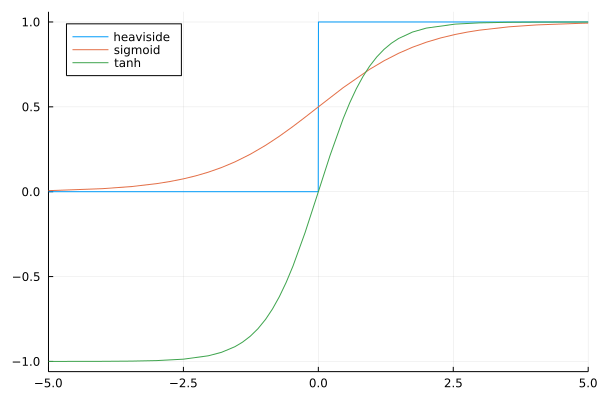
\includegraphics[scale=0.25]{ann_activation_01.png}
    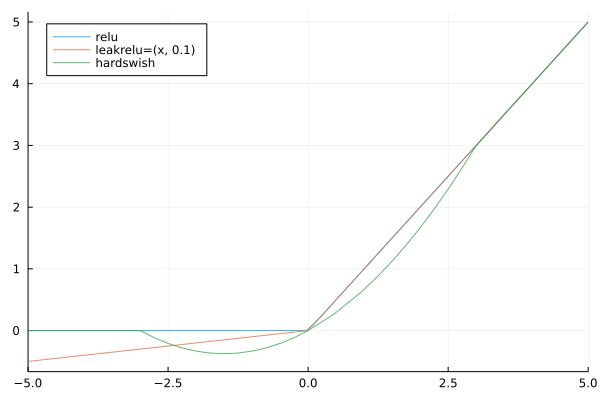
\includegraphics[scale=0.25]{ann_activation_02.png}
    \caption{A visual comparison between the outputs of Heaviside, sigmoid, tanh, \gls{ReLU}, Leaky ReLU, and hard swish activation functions}
    \label{fig:heaviside-sigmoid-tanh}
\end{figure}

To solve the vanishing gradients problem, the \gls{ReLU} activation function is used
\begin{equation*}
    \phi(z) = max(0, z).
\end{equation*}
One disadvantage of this activation function is the dying \gls{ReLU} problem, which is when the node's output gets close to zero or is negative.
When that happens, the gradients of the loss function with respect to the parameter for that node are zero, causing the node to stop learning.
A function that addresses this issue is the Leaky \gls{ReLU} activation
\begin{equation*}
    \phi(z) = max(\alpha z, z),
\end{equation*}
where $\alpha$ is a hyperparameter that can be chosen to define negative output values of the function.
Or the hard swish activation function \cite{howardSearchingMobileNetV32019}
\begin{equation*}
\phi(z)=\begin{cases}
    0 & \text{if}\ z \leq -3 \\
    z & \text{if}\ z \geq 3 \\
    z * (z + 3) / 6 & \text{otherwise}  \\
\end{cases}
\end{equation*}